\documentclass{article}
\usepackage{graphicx}
\usepackage{hyperref}


\title{Programmentwurf für Check-Mate}
\author{Moritz Knapp  \\
	SICK AG  \\
	\and 
	David Schmidt \\
	SICK AG \\
	}

\date{\today}
\begin{document}

\maketitle

\tableofcontents
\newpage

\section{Intro}

Da wir, David und Moritz, schon immer gerne Schach gegeneinander spielten um auch in Lernpausen unseren Geist nicht zu unterfordern, entschieden wir uns ein eigenes Schach zu programmieren. 
Zudem sind wir davon überzeugt, dass Schach eine perfekte Grundlage für objektorientiertes Programmieren bietet, aufgrund der vielen Figuren die jeweils gerade und schräge Züge individuell ausführen.

\section{Clean-Architecture} \label{sec:cleanArc}
Bereits vor dem Studium hat David schonmal ein Schach programmiert. Dabei handelte es sich um ca 3000 Zeilen hochineffizienten Arduino Code. In diesem Projrekt wollten wir unseren früheren Ichs beweisen wie viel eleganter so etwas umsetzbar ist. Der erste Schritt dazu ist die Clean-Architecture.

\begin{figure}[h]
	\begin{center}
		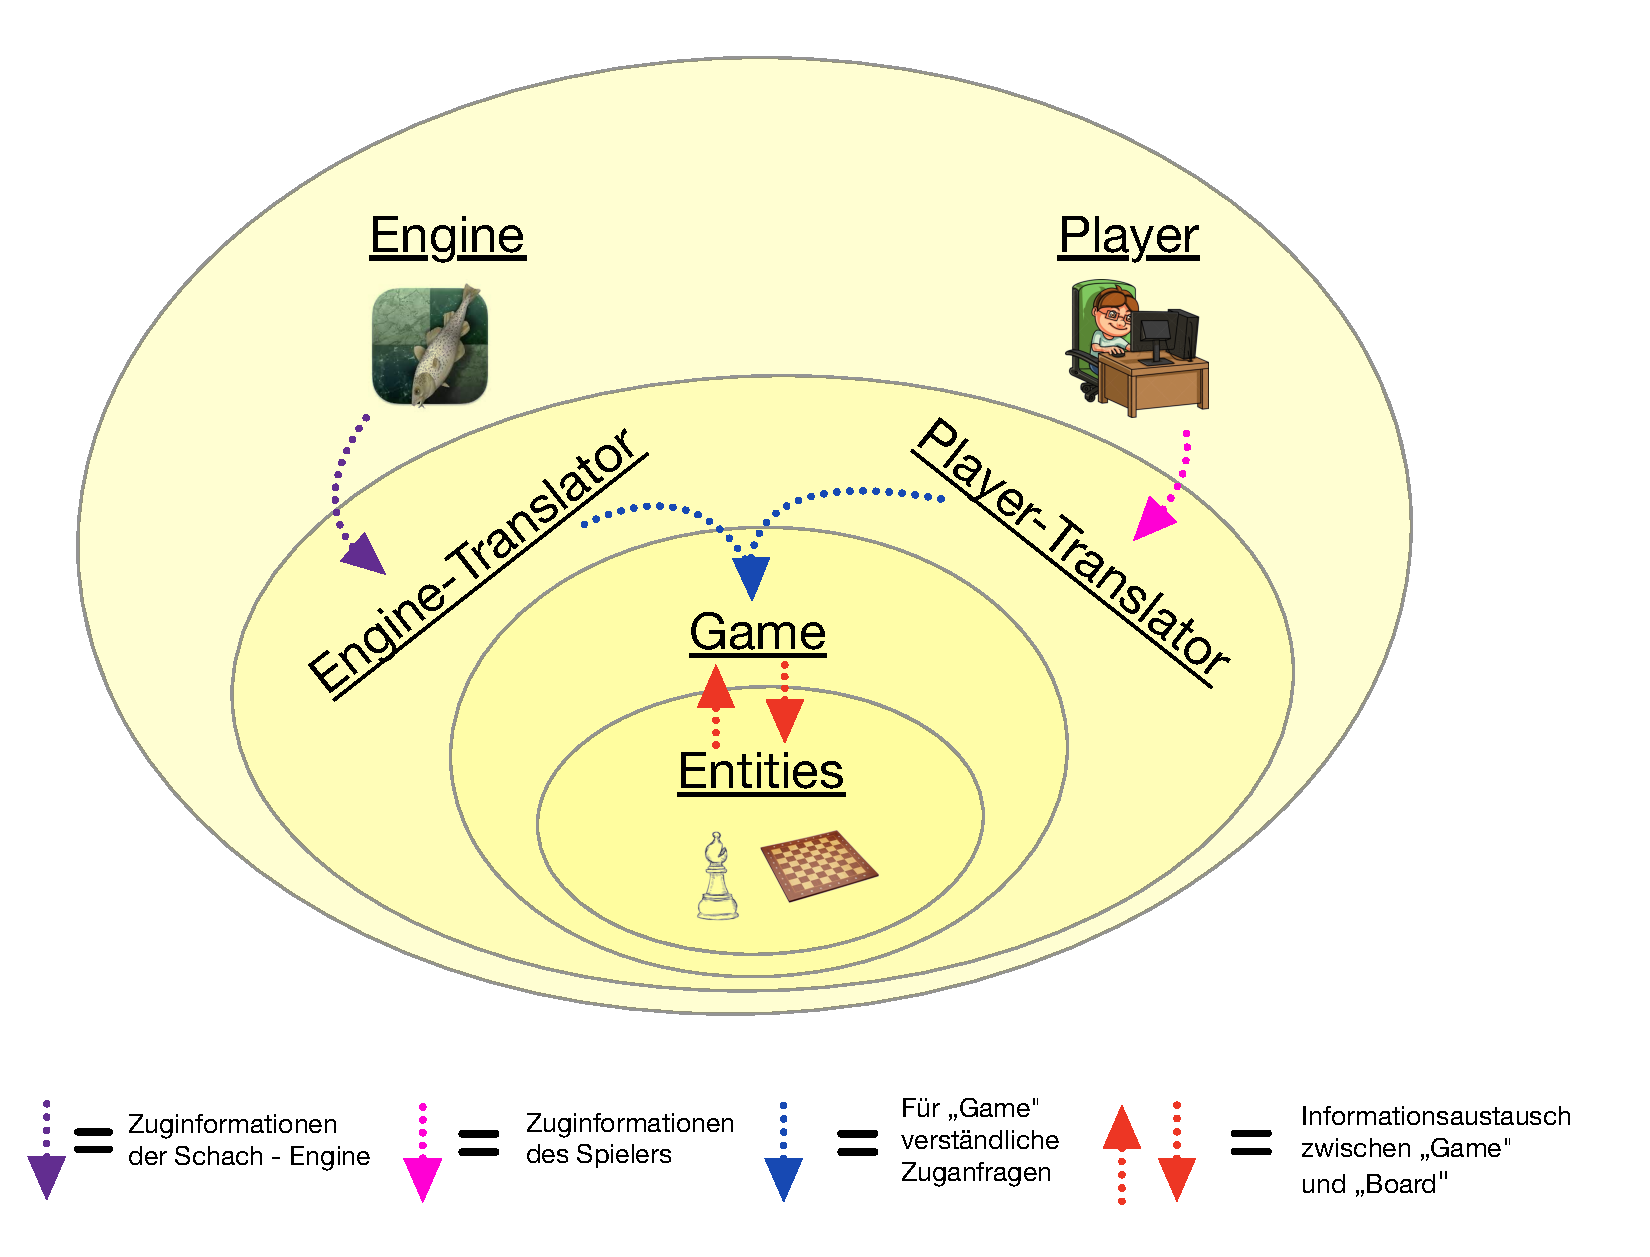
\includegraphics[width = \textwidth]{onion.pdf}
		\caption{Übersicht über die Clean Architecture}
	\end{center}
\end{figure}

Zusammengefasst ermöglicht eine Clean Architecture die Veränderung der Umgebung, bzw. des Systems, ohne den eigentlichen Kern des Codes anpassen zu müssen.
Das bedeutet, dass wir theoretisch unser Spiel um ein echtes Spielbrett mit LEDs und Arduino- Raspberry-Steuerung erweitern könnten, ohne unseren Schach-Code zu verädnern.

\subsection{Schicht 1: Entitys}
Die Entitys sind der Kern unseres Spiels. Unabhängig von der Umgebung sind die einzelnen Figuren virtuell auf einem Feld positioniert und können umplatziert werden.
Dadurch ergeben sich grundlegend Folgende Klassen: 

\begin{center}
	\begin{itemize}
		\item Board
		\item Square
		\item Piece
	\end{itemize}
\end{center}

Ein Board besteht aus vielen Squares, auf denen jeweils ein Piece stehen kann. Um dies zu implementieren und später auch verschiedene Pieces zu benutzen, zeigt \autoref{pic:umlEntitys} alle Klassen welche unser Kern der Clean-Architektur beinhalten soll. 
\newpage
\begin{figure}[h]
	\begin{center}
		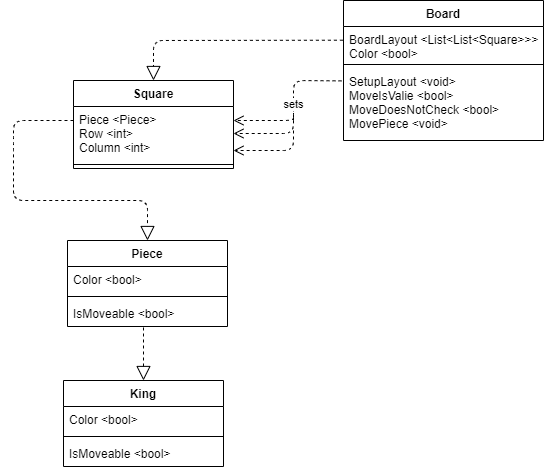
\includegraphics[width=10cm]{entitys.png}
		\caption{\label{pic:umlEntitys} UML-Diagramm der Entitys}
	\end{center}
\end{figure}
Das Diagramm zeigt die Schach-Logik im Kern unserer Clean Architecture, bzw. die Entitys. Das \texttt{Board} stellt das Schachbrett dar. Dieses besteht aus 64 \texttt{Squares}. Die Methode \texttt{SetupLayout} erstellt das Board und besetzt die richtigen Felder mit Pieces mit der entsprechenden Farbe.
Von den eigentlichen \texttt{Pieces} ist hier nur der König gezeigt, da die anderen Figuren genau wie er die Methode \texttt{IsMoveable} implementieren. 
Das Board bietet drei Methoden, von denen nur eine tatsächlich von weiteren Schichten verwendet wird: \texttt{MovePiece}. Die Methode überprüft mit \texttt{MoveIsVali} ob es sich um einen Validen Zug handelt. \texttt{MoveIsValid} ruft dabei die von Figuren implementierte Methode \texttt{IsMoveable} auf um zu überprüfen ob die Figur theoretisch in der Lage wäre den Zug durchzuführen.\\ Der wesentliche Unterschied zwischen \texttt{MoveIsValid} und \texttt{IsMoveable} besteht darin, dass Figuren das Board nicht kennen und auch nicht wissen wo sie sich befinden. \texttt{IsMoveable} signalisiert lediglich, ob ein Zug rein von den allgemeinen Zugmöglichkeiten der Figur möglich ist (zB. Läufer kann nur schräg laufen). \texttt{MoveIsValid} ist eine Methode des Boards und kann somit auch situationsbedingte Auskunft über die Validität des Zuges geben. Wenn die Figur \texttt{IsMoveable} ist, wird von \texttt{MoveIsValid} noch überprüft ob weitere Figuren im Weg stehen und der Zug sich selbst in Schach setzen würde (\texttt{MoveDoesNotCheck}). Ist alles überprüft, wird der Zug durchgeführt.

\subsection{Schicht 2: Use-Case}
Die Use-Cases bilden die zweite Schicht der Clean Architekture. Sie können informationen der ersten Schicht erhalten (Entitys), diese sind aber nicht abhängig von den Use-Cases.\\
In unserem Fall haben wir nur einen Use-Case: Das Spiel, bzw. \texttt{Game}. Diese Klasse erstellt das Board, bzw ruft die Funktion \texttt{SetupLayout} auf, hat aber noch weitere Informationen die über das einfache Ziehen von Figuren hinausgehen:
\begin{center}
	\begin{itemize}
		\item Spielerposition (z.B. Spieler 1 spielt unten),
		\item Spielerfarbe (z.B. Spieler 1 ist weiß)
		\item und aktueller Spieler (z.B. Spieler 1 ist dran).
	\end{itemize}
\end{center}
Der Use-Case initialisiert das Board, wodurch die Farbe des unten spielenden Spielers zufällig gewählt wird. Logisch betrachtet spielt für das \texttt{Game} Spieler 1 in jedem Fall \textit{unten}. Da immer weiß beginnt, ist es zufällig ob Spieler 1 beginnen darf oder nicht. Welche Art von User-Interface nun Spieler 1 steuert, ist Aufgabe der dritten Schicht, welche in unserem Fall den Menschen an der Gui Spieler 1 und eine Schach-Engine Spieler 2 zuordnet. \texttt{Game} ist von dieser Information jedoch abgekapselt, da eine Zuganfrage in jedem Fall gleich aussieht.
So eine Anfrage ist von \texttt{Game} definiert (z.B. 'e5,e6' = ''Zug von e5 nach e6''). \\
Wird nun eine solche Anfrage gestellt, verlangt \texttt{Game} von \texttt{Board} eine Auskunft über die Farbe der Figur, welche sich auf dem \textit{von}-Feld befindet. Stimmt diese mit der Farbe des aktuell spielenden Spielers überein, kann der Zug nach Validitätsprüfung ausgeführt werden. Anhand dessen ob \texttt{MovePiece} \texttt{true} oder \texttt{false} zurückgibt, ist der andere Spieler daraufhin am Zug, oder nicht.
\subsection{Schicht 3: Übersetzer}
Sollte es dazu kommen, dass die Umgebung beispielsweise zu einer Ascii-Oberfläche geändert wird, müssen ab dieser Schicht Veränderungen am Code erfolgen. Solange jedoch die Zug-Anfragen richtig gestellt werden, arbeitet der Code in den unteren Schichten immer gleich. In der 3. Schicht befindet sich ein GUI- und Engine-Translator. Diese übersetzen Züge von Spieler und Engine und geben sie richtig Codiert an die zweite Schicht. solche Zug-Anfragen können völlig asynchron erfolgen, sie führen jedoch zu nichts, falls der Zug nicht den Regeln entspricht, oder der Spielende nicht am Zug ist.
\subsection{Schicht 4: User-Interfaces}
Auf dieser Ebene befinden sich die Interfaces für die Spieler. In unserem Fall sind das die GUI und die Schachengine. %David schreib was zur enginge hier ich hab kp
Die GUI stellt das Schachbrett grafisch dar und bietet die Möglichkeit durch anklicken von Feldern Figuren zu ziehen (z.B. erster Klick auf \textit{E2}, zweiter Klick auf \textit{E3} $\Rightarrow$ \textit{E2 nach E3}). Diese Klicks werden von Schicht 3 für das Spiel übersetzt.


\section{Programmierprizipien}
\subsection{pros/cons/wieso wir?}
\subsection{SOLID}
\subsubsection{Single Resposibility Principle}
\subsubsection{Open/Closed Principle}
\subsubsection{Liskov' Substitution Principle}
\subsubsection{Interface Segregation Principle}
\subsubsection{Dependency Inversion Principle}
Auf Translator anwenden
\subsection{GRASP}
\subsubsection{Low Coupling}
\subsubsection{High Cohesion}
\subsection{DRY (Don't Repeat Yourself)}
Schon umgesetzt?


\section{Unit Testing}
\subsection{pros/cons/wieso wir?}
\subsection{ATRIP}
\subsection{Code Coverage}
\subsection{Mocking}

\section{Refactoring}
\subsection{Beispiele und Begründungen}
\subsection{Code Smells}

\section{Entwurfsmuster}
\subsection{Diagramme und Begründungen}

\section{Fazit}\label{sec:end}

\end{document}